\documentclass[a4paper,landscape]{article}
\usepackage{fullpage}
\usepackage{tikz}
\usetikzlibrary{calc}
\pagestyle{empty}
\begin{document}
\vbox to 1em{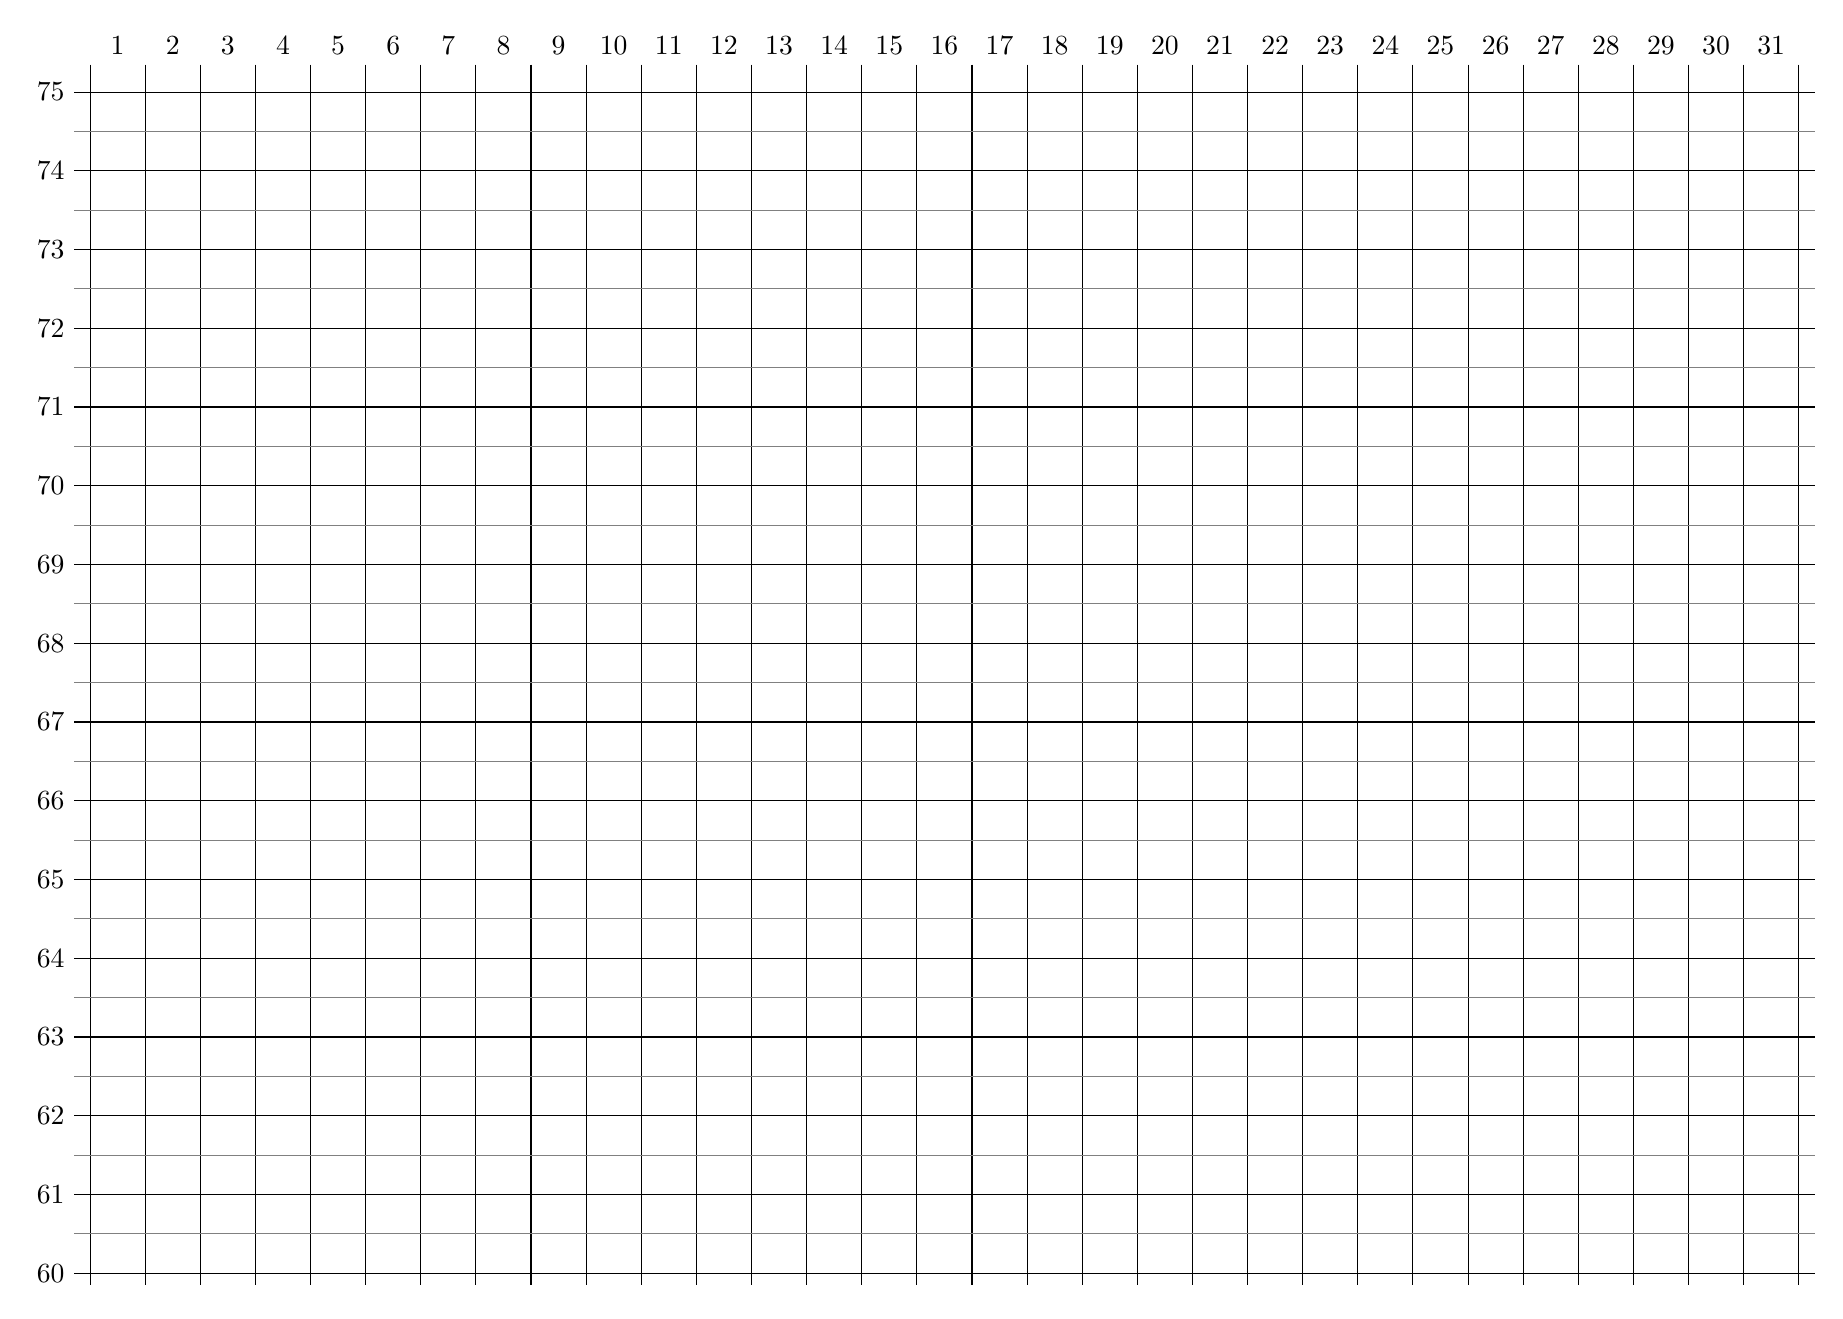
\begin{tikzpicture}
\foreach \x in {1,...,31} {
	\draw ($ 0.7*(\x,0.5) $) coordinate (X) -- ++(0,-15.5);
	\draw (X) ++(0.35,0) node[above] {\x};
}
\draw ($ 0.7*(32,0.5) $) coordinate (X) -- ++(0,-15.5);
\foreach \y in {60,...,75} {
	\draw ($ (0.5,\y) - (0,75) $) node[left] {\y} -- ++(+22.1,0);
}
\foreach \y in {61,...,75} {
	\draw[gray] ($ (0.5,\y) - (0,75.5) $) -- ++(+22.1,0);
}
\end{tikzpicture}}
\end{document}
